% (The MIT License)
%
% Copyright (c) 2023 Yegor Bugayenko
%
% Permission is hereby granted, free of charge, to any person obtaining a copy
% of this software and associated documentation files (the 'Software'), to deal
% in the Software without restriction, including without limitation the rights
% to use, copy, modify, merge, publish, distribute, sublicense, and/or sell
% copies of the Software, and to permit persons to whom the Software is
% furnished to do so, subject to the following conditions:
%
% The above copyright notice and this permission notice shall be included in all
% copies or substantial portions of the Software.
%
% THE SOFTWARE IS PROVIDED 'AS IS', WITHOUT WARRANTY OF ANY KIND, EXPRESS OR
% IMPLIED, INCLUDING BUT NOT LIMITED TO THE WARRANTIES OF MERCHANTABILITY,
% FITNESS FOR A PARTICULAR PURPOSE AND NONINFRINGEMENT. IN NO EVENT SHALL THE
% AUTHORS OR COPYRIGHT HOLDERS BE LIABLE FOR ANY CLAIM, DAMAGES OR OTHER
% LIABILITY, WHETHER IN AN ACTION OF CONTRACT, TORT OR OTHERWISE, ARISING FROM,
% OUT OF OR IN CONNECTION WITH THE SOFTWARE OR THE USE OR OTHER DEALINGS IN THE
% SOFTWARE.

\documentclass{article}
\usepackage[T1]{fontenc}
\usepackage[utf8]{inputenc}
\usepackage[nocn,nonumbers,noframes,sf,bold]{ffcode}
\usepackage[static]{clicks}
\usepackage{tikzsymbols}
\usepackage{booktabs}
\usetikzlibrary{positioning}
\usepackage[increment]{crumbs}
\usepackage[template,scheme=light,nominutes]{ppt-slides}
\usepackage{href-ul}
\usepackage{svg}
\usepackage{soul}
\usepackage{doi}
\usepackage{qrcode}
\renewcommand{\ttdefault}{cmtt}
\newcommand\nospell[1]{#1}
\newcommand*{\thetitle}{Open Source Kung-Fu}
\newcommand*{\thesubtitle}{Nine Levels of It}
\newcommand*{\theauthor}{Yegor Bugayenko}
\pptLeft{
\includegraphics[height=1.4em]{neimark-logo.png}\\[.6em] October 18th, 2024}
\pptRight{@yegor256}

\newcounter{level}
\newcommand\level[1]{\stepcounter{level}\plush{\pptThought{{\scshape\sffamily \textcolor{orange}{Level \thelevel}:} #1.}}}

\newcommand\pitch[1]{\plush{\begin{pptMiddle} #1 \end{pptMiddle}}}
\newcommand\qte[4][]{
  \pitch{
    \pptQuote
      [\scriptsize\scshape\color{gray}{#1}]
      {#2.jpg}
      {#3}
      {\color{gray}\rmfamily\scriptsize\bibentry{#4}}
  }
}
\newcommand\source[1]{\par{\scriptsize\color{gray} Source: \bibentry{#1}\par}}

\AtBeginDocument{%
  \pptLeft{\thetitle{}}%
  \pptRight{@yegor256}%
  \nobibliography*
  \bibliographystyle{plainnat}
}

\RequirePackage{bibentry}
\RequirePackage{natbib}
\AtEndDocument{%
  \begin{multicols}{2}
  \setlength{\bibsep}{.2em}
  \renewcommand{\bibfont}{\scriptsize}
  \bibliography{main}
  \end{multicols}
}

\begin{document}

\plush{
  \begin{pptMiddle}
    % 
\includegraphics[height=2.6em]{neimark-logo.png}
    \pptTitle{\thetitle}{\thesubtitle}\par
    {\scshape \theauthor}
    \newline
    {\small Zerocracy\par}
  \end{pptMiddle}
}

\pitch{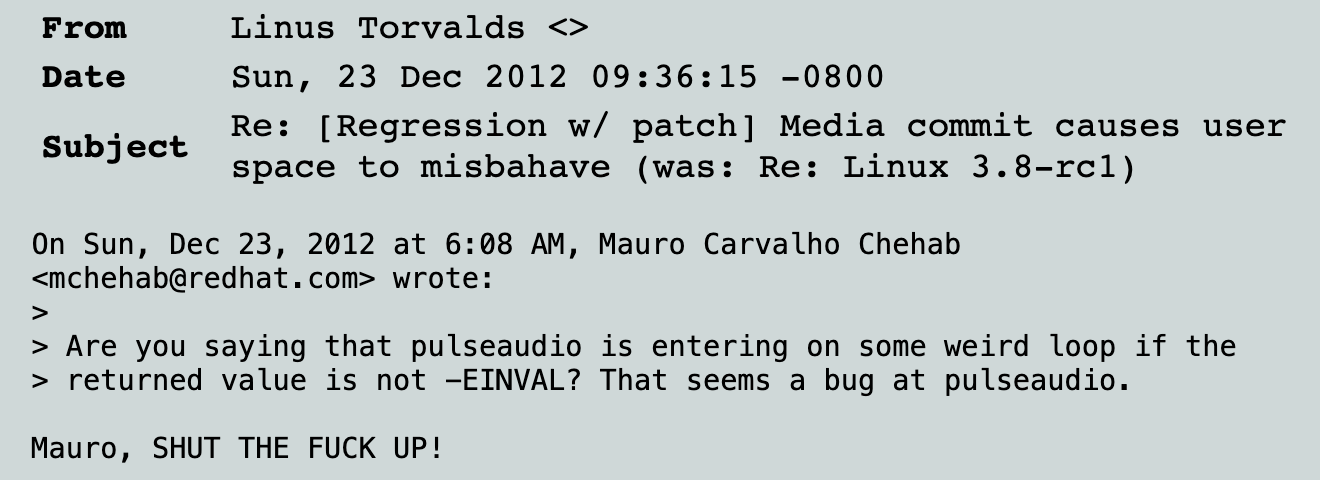
\includegraphics[width=.95\linewidth]{linus-email.png}}

\qte
  [\nospell{Isabella Ferreira}]
  {isabella-ferreira}
  {We conducted a qualitative analysis on 1,545 emails from the Linux Kernel Mailing List that were associated with rejected changes. We found that \ul{more than half} (67\%) of the non-technical emails included uncivil features. Particularly, frustration, name calling, and impatience are the most frequent features in uncivil emails. }
  {ferreira2021shut}

\level{You've got your own GitHub account}

\qte
  [\nospell{Kristine Nowak}]
  {kristine-nowak}
  {Avatars that were more \ul{anthropomorphic} were perceived to be more \ul{attractive} and \ul{credible}. The strongest predictor of these variables, however, was the degree of masculinity or femininity (lack of androgyny) of an avatar.}
  {nowak2005influence}

\pitch{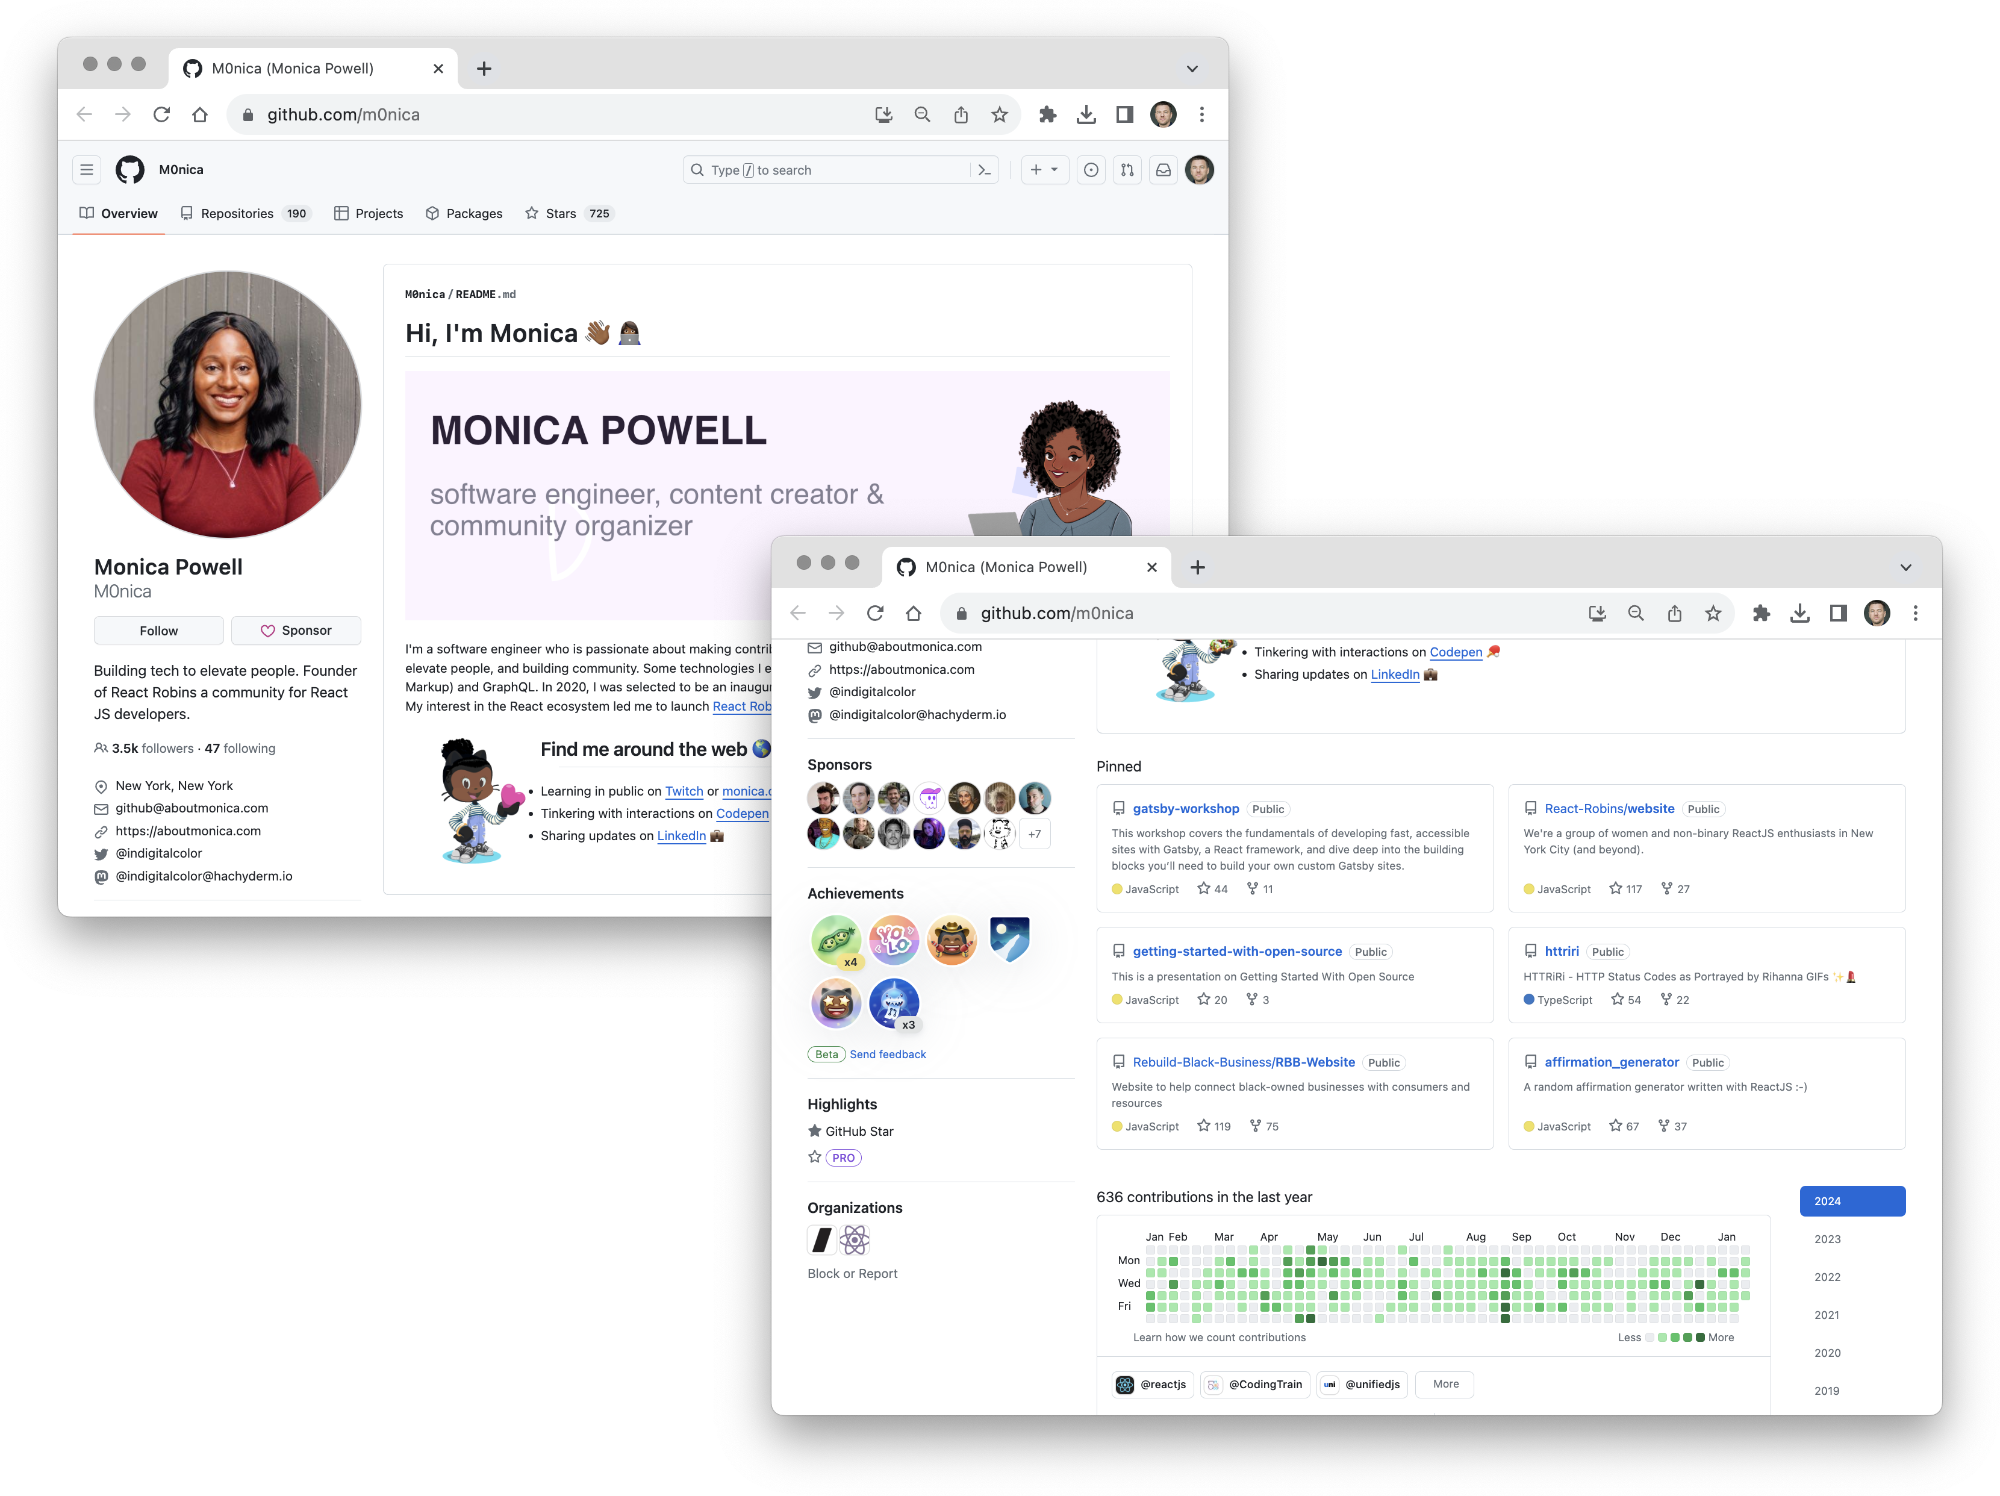
\includegraphics[width=.75\linewidth]{monica.png}}

\level{Your pull request has been merged}

\qte
  [\nospell{\nospell{Bram Adams}}]
  {bram-adams}
  {We found that \ul{33\%} of the patches makes it into a Linux release, and that most of them need \ul{3 to 6 months} for this.}
  {jiang2013will}

\qte
  [\nospell{Jacek Czerwonka}]
  {jacek-czerwonka}
  {Only about 15\% of comments provided by reviewers indicate a possible defect, much less a blocking defect. Rather, it is feedback related to the long-term code \ul{maintainability} that comprises a much larger portion of comments provided by reviewers; at least 50\% of all.}
  {czerwonka2015code}

\qte
  [\nospell{Caitlin Sadowski}]
  {caitlin-sadowski}
  {A correlation between \ul{change size} and \ul{review quality} is acknowledged by Google and developers are strongly encouraged to make small, incremental changes (with the exception of large deletions and automated refactoring).}
  {sadowski2018modern}

\qte
  [\nospell{Carolyn D. Egelman}]
  {carolyn-egelman}
  {Google categorizes CRs into specific sizes, these sizes are indicated as part of the code review tool and in the notification to the reviewer of the code change... The general advice is to \ul{split} change requests for \ul{easier} and \ul{quicker} reviews when possible.}
  {egelman2020predicting}

\qte
  [\nospell{Marco Ortu}]
  {marco-ortu}
  {Our results show that \ul{valence} (expressed in comments received and posted by a reporter) and \ul{joy} expressed in the comments written by a reporter are linked to a \ul{higher likelihood} of issues to be merged. On the contrary, sadness, anger, and arousal expressed in the comments written by a reporter, and anger, arousal, and dominance expressed in the comments received by a reporter, are linked to a lower likelihood of a pull request to be merged.}
  {ortu2020you}

\qte
  [\nospell{Valentina Lenarduzzi}]
  {valentina-lenarduzzi}
  {Unexpectedly, quality \ul{flaws} measured by PMD turned out not to affect the acceptance of a pull request at all. As suggested by other works, other factors such as the \ul{reputation} of the maintainer and the \ul{importance} of the delivered feature might be more important than other qualities in terms of pull request acceptance.}
  {lenarduzzi2021does}

\level{You've published a package}

\level{You've received a pull request}

\qte
  [Simon Weber]
  {simon-weber}
  {Upon investigation, popular projects were found to have larger READMEs (median 2 kilobytes vs. 500 bytes). Also, 95\% of popular projects have nonempty READMEs, compared to only 65\% of unpopular projects.}
  {weber2014makes}

\qte
  [\nospell{Asher Trockman}]
  {asher-trockman}
  {We find that non-trivial \ul{badges}, which display the build status, test coverage, and up-to-dateness of dependencies, are mostly reliable signals, correlating with more tests, better pull requests, and fresher dependencies.}
  {trockman2018adding}

\qte
  [\nospell{Shaowei Wang}]
  {shaowei-wang}
  {The frequency/number of readme \ul{updates} and the number of \ul{lists} and \ul{links} positively correlate with the likelihood of a repository being popular.}
  {wang2023study}

\level{Your repository's been taken over}

\plush{
  \begin{multicols}{2}
  \pptPic{.9}{micromap.png}
  \par\columnbreak\par
  \pptPic{.9}{benchmark.png}
  \end{multicols}
  Thanks to \href{https://github.com/zefick}{@Zefick}!}

\level{Your repository's got 100 bugs}

\qte
  [\nospell{Myers, Glenford J.}]
  {glenford-myers}
  {You cannot test a program to guarantee that it is error free... It is impractical, often impossible, to find \ul{all} the errors in a program.}
  {myers2012art}

\qte
  [\nospell{Reis Christian}]
  {reis-christian}
  {Though it commonly has a prejorative connotation, in the Mozilla Project the term \textbf{bug} is used to refer to any field request for modification in the software, be it an \ul{actual} defect, an enhancement, or a change in functionality. (``bug-driven development'')}
  {reis2002overview}

\pitch{\pptBanner{Repositories With a Lot of Bugs (9 Feb 2024)}
{\small\begin{tabular}{lr}
\toprule
Github Repository & Bugs \\
\midrule
\href{https://bugzilla.mozilla.org/}{mozilla} & 1,8M+ \\
\href{https://gitlab.com/gitlab-org/gitlab/-/issues}{\texttt{gitlab-org/gitlab}} & 172,462 \\
\href{https://github.com/flutter/flutter}{\texttt{flutter/flutter}} & 79,386 \\
\href{https://github.com/kubernetes/kubernetes}{\texttt{kubernetes/kubernetes}} & 42,627 \\
\href{https://github.com/tensorflow/tensorflow}{\texttt{tensorflow/tensorflow}} & 36,776 \\
\href{https://github.com/moby/moby}{\texttt{moby/moby}} & 19,367 \\
\bottomrule
\end{tabular}}\par
All repositories are open source.}

\level{Google's offered to put you on a retainer}

\plush{\pptPic{.9}{github-email.png}}

\level{GitHub's offered you large runners, for free}

\plush{
  \begin{multicols}{2}
  \pptPic{.9}{alexander.png}\par
  Watch the interview \href{https://www.youtube.com/watch?v=xMGNlUZQ-6w}{on YouTube}.\par
  \qrcode[height=4em]{https://www.youtube.com/watch?v=xMGNlUZQ-6w}
  \par\columnbreak\par
  \textcolor{orange}{Alexander Medvednikov}, the creator of the \href{https://vlang.io/}{V programming language},
  in the interview mentioned that GitHub offers his project free access
  to larger CI/CD resources (aka ``\textcolor{orange}{large runners}'').\par
  
\includegraphics[width=3em]{v-logo.png}\par
  \href{https://vlang.io/}{www.vlang.io}
  \end{multicols}}

\level{You've got \$100K/year from GitHub sponsors}

\plush{
  \begin{multicols}{2}
  \pptPic{.9}{sponsors-1.png}\par
  Read the story of \href{https://github.com/calebporzio}{\textcolor{orange}{Caleb Porzio}},
  and \href{https://github.com/readme/stories/caleb-porzio}{this one} too.\par
  He is the creator of \href{https://github.com/livewire/livewire}{LiveWire} (22K\(\star\))
  and \href{https://github.com/alpinejs/alpine}{AlpineJS} (28K\(\star\)).
  \par\columnbreak\par
  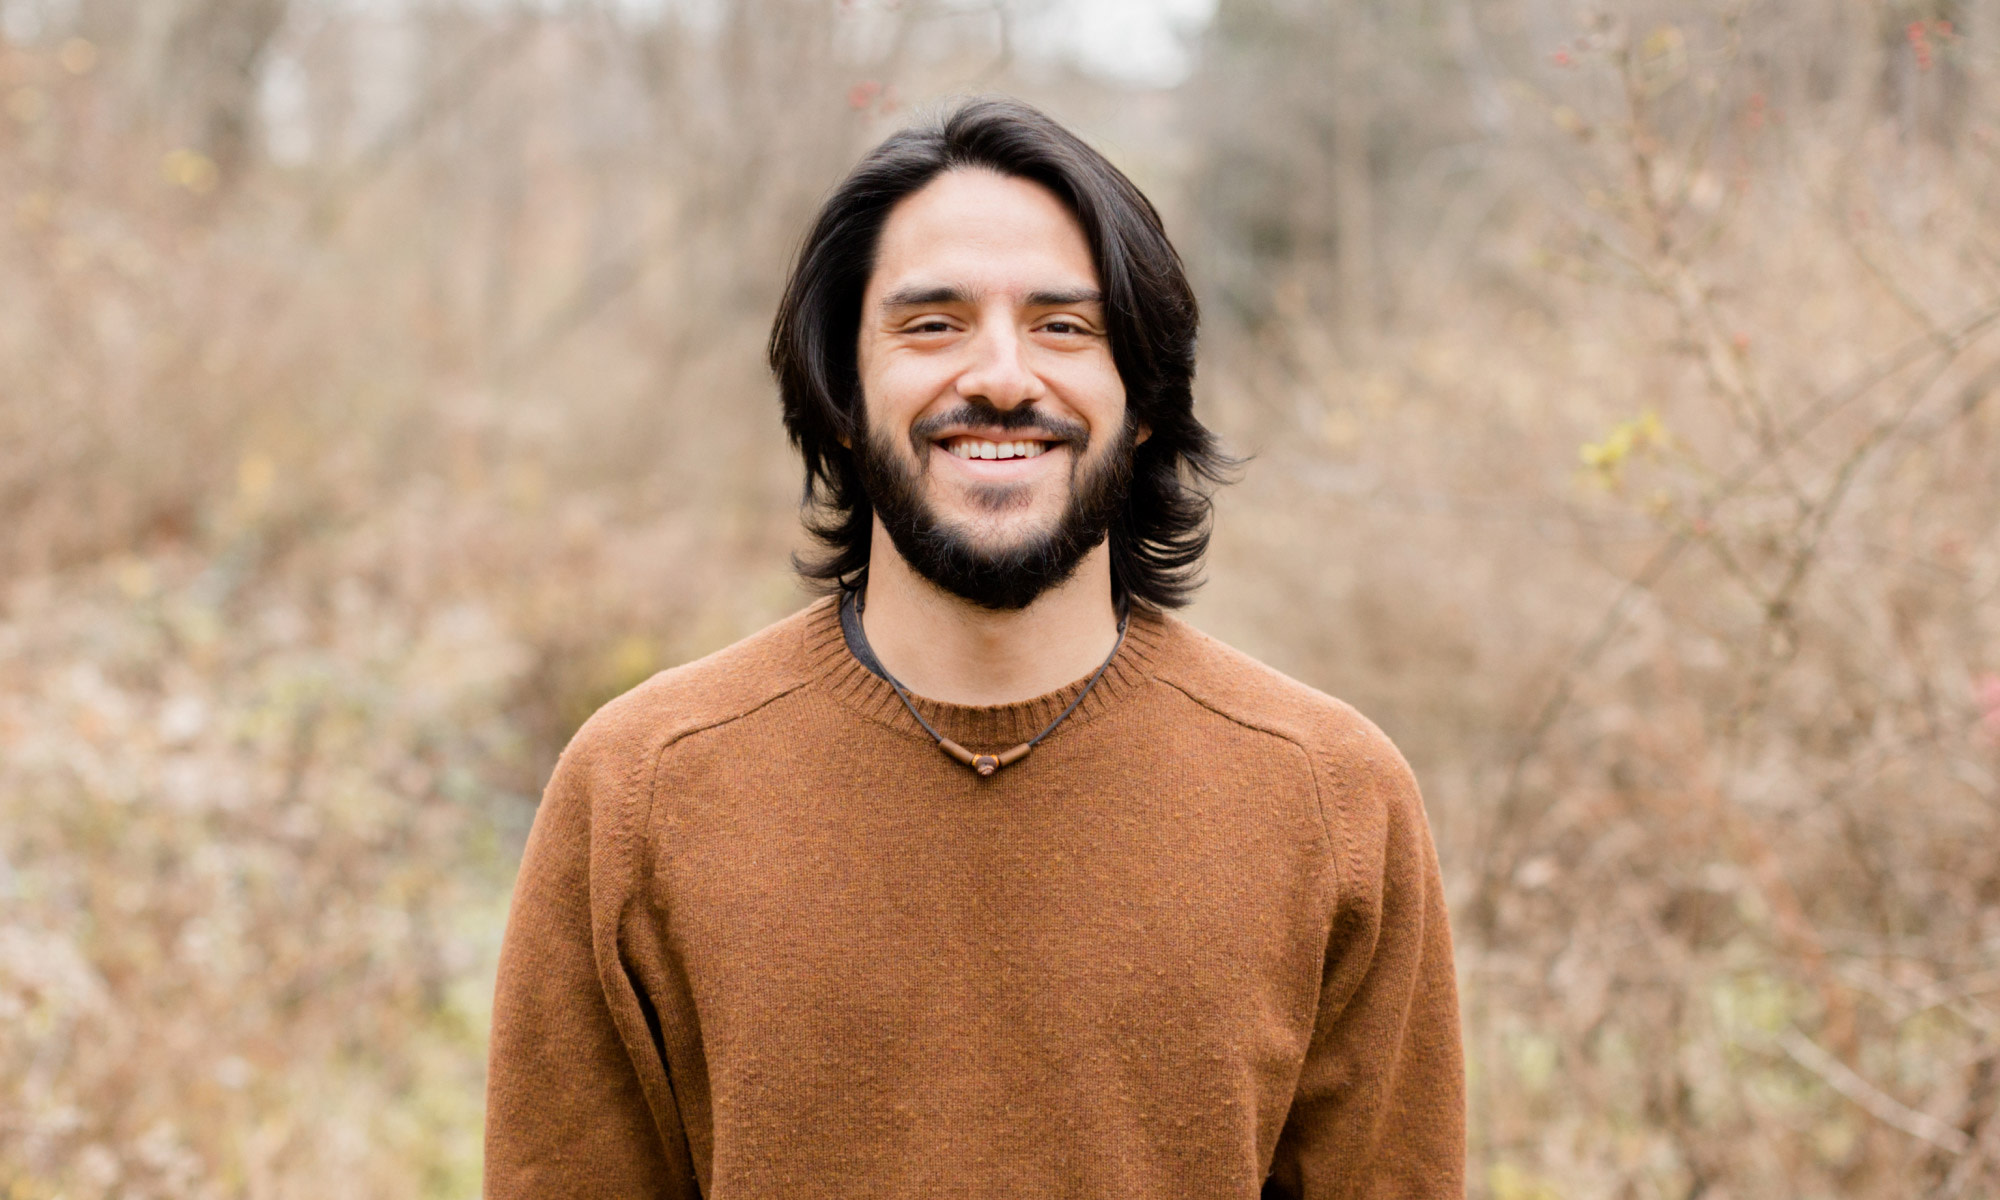
\includegraphics[width=\linewidth]{caleb-porzio.jpg}\par
  \pptPic{.9}{sponsors-2.png}
  \end{multicols}}

\plush{
  \begin{multicols}{2}
  \pptBanner{My Telegram Channel:}\par
  \qrcode[height=7em]{https://t.me/yegor256news}\par
  \href{https://t.me/yegor256news}{\texttt{@yegor256news}}
  \par\columnbreak\par
  \pptBanner{``Open Source Best Practices''}\par
  Eight Lectures for Innopolis University:\par
  \qrcode[height=7em]{https://www.youtube.com/playlist?list=PLaIsQH4uc08zjutyoBOtoa6fnxzrCQK2Q}\par
  \href{https://www.youtube.com/playlist?list=PLaIsQH4uc08zjutyoBOtoa6fnxzrCQK2Q}{\texttt{PlayList}}
  \end{multicols}}

\plush{}

\end{document}
